\documentclass{standalone}
\usepackage{tikz}
\usetikzlibrary{patterns, positioning}

\begin{document}
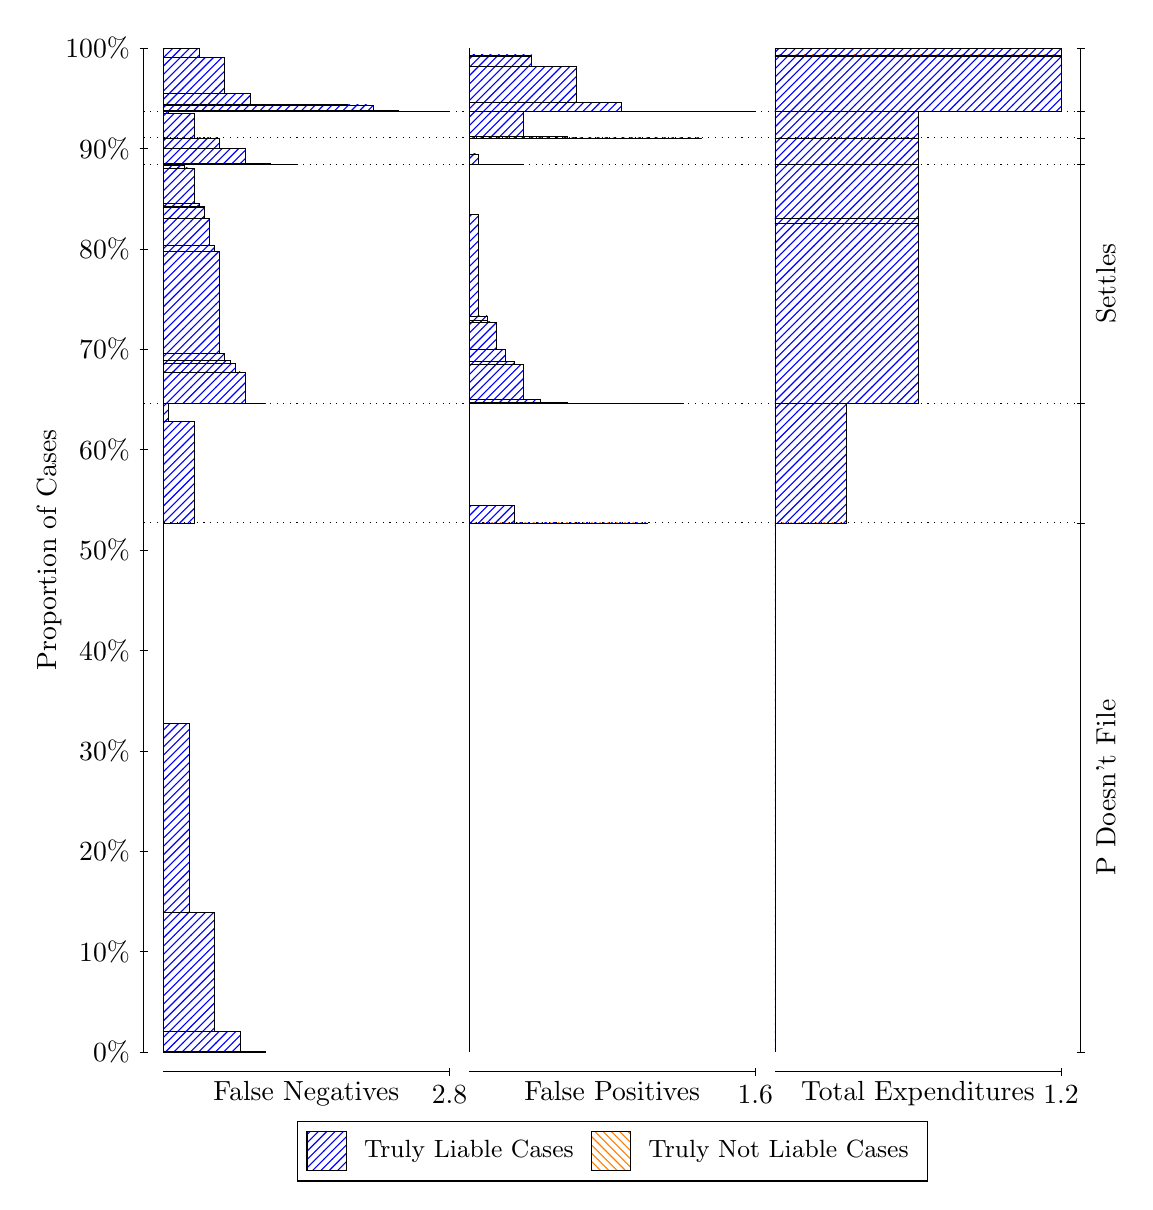
\begin{tikzpicture}
\draw[black, very thin] (1.5,1.75) -- (1.5,14.5);
\node[rotate=90, anchor=center] at (0.3, 8.125) {Proportion of Cases};
\draw[black, very thin] (1.45,1.75) -- (1.55,1.75);
\node[anchor=east] at (1.45, 1.75) {0\%};
\draw[black, very thin] (1.45,3.025) -- (1.55,3.025);
\node[anchor=east] at (1.45, 3.025) {10\%};
\draw[black, very thin] (1.45,4.3) -- (1.55,4.3);
\node[anchor=east] at (1.45, 4.3) {20\%};
\draw[black, very thin] (1.45,5.575) -- (1.55,5.575);
\node[anchor=east] at (1.45, 5.575) {30\%};
\draw[black, very thin] (1.45,6.85) -- (1.55,6.85);
\node[anchor=east] at (1.45, 6.85) {40\%};
\draw[black, very thin] (1.45,8.125) -- (1.55,8.125);
\node[anchor=east] at (1.45, 8.125) {50\%};
\draw[black, very thin] (1.45,9.4) -- (1.55,9.4);
\node[anchor=east] at (1.45, 9.4) {60\%};
\draw[black, very thin] (1.45,10.675) -- (1.55,10.675);
\node[anchor=east] at (1.45, 10.675) {70\%};
\draw[black, very thin] (1.45,11.95) -- (1.55,11.95);
\node[anchor=east] at (1.45, 11.95) {80\%};
\draw[black, very thin] (1.45,13.225) -- (1.55,13.225);
\node[anchor=east] at (1.45, 13.225) {90\%};
\draw[black, very thin] (1.45,14.5) -- (1.55,14.5);
\node[anchor=east] at (1.45, 14.5) {100\%};

\draw[black, very thin] (13.4,1.75) -- (13.4,14.5);
\draw[black, very thin] (13.35,1.75) -- (13.45,1.75);
\node[anchor=west] at (13.35, 1.75) {};
\draw[black, very thin] (13.35,8.4689) -- (13.45,8.4689);
\node[anchor=west] at (13.35, 8.4689) {};
\draw[black, very thin] (13.35,9.9867) -- (13.45,9.9867);
\node[anchor=west] at (13.35, 9.9867) {};
\draw[black, very thin] (13.35,13.025) -- (13.45,13.025);
\node[anchor=west] at (13.35, 13.025) {};
\draw[black, very thin] (13.35,13.36) -- (13.45,13.36);
\node[anchor=west] at (13.35, 13.36) {};
\draw[black, very thin] (13.35,13.693) -- (13.45,13.693);
\node[anchor=west] at (13.35, 13.693) {};
\draw[black, very thin] (13.35,14.5) -- (13.45,14.5);
\node[anchor=west] at (13.35, 14.5) {};

\draw[black, very thin, pattern color=blue, pattern=north east lines] (1.75,1.75) rectangle (3.0476,1.7526);
\draw[black, very thin, pattern color=blue, pattern=north east lines] (1.75,1.7526) rectangle (2.7232,2.011);
\draw[black, very thin, pattern color=blue, pattern=north east lines] (1.75,2.011) rectangle (2.3988,3.5205);
\draw[black, very thin, pattern color=blue, pattern=north east lines] (1.75,3.5205) rectangle (2.0744,5.9204);
\draw[black, very thin, pattern color=orange, pattern=north west lines] (1.75,5.9204) rectangle (1.75,5.9204);
\draw[black, very thin, pattern color=blue, pattern=north east lines] (1.75,5.9204) rectangle (1.75,8.4689);
\draw[black, very thin, pattern color=blue, pattern=north east lines] (1.75,8.4689) rectangle (2.1393,9.7603);
\draw[black, very thin, pattern color=blue, pattern=north east lines] (1.75,9.7603) rectangle (1.8149,9.9858);
\draw[black, very thin, pattern color=orange, pattern=north west lines] (1.75,9.9858) rectangle (1.75,9.9858);
\draw[black, very thin, pattern color=blue, pattern=north east lines] (1.75,9.9858) rectangle (1.75,9.9867);
\draw[black, very thin, pattern color=blue, pattern=north east lines] (1.75,9.9867) rectangle (3.0476,9.9867);
\draw[black, very thin, pattern color=blue, pattern=north east lines] (1.75,9.9867) rectangle (2.9179,9.9869);
\draw[black, very thin, pattern color=blue, pattern=north east lines] (1.75,9.9869) rectangle (2.7881,10.384);
\draw[black, very thin, pattern color=blue, pattern=north east lines] (1.75,10.384) rectangle (2.7232,10.387);
\draw[black, very thin, pattern color=blue, pattern=north east lines] (1.75,10.387) rectangle (2.6583,10.495);
\draw[black, very thin, pattern color=blue, pattern=north east lines] (1.75,10.495) rectangle (2.5935,10.532);
\draw[black, very thin, pattern color=blue, pattern=north east lines] (1.75,10.532) rectangle (2.5286,10.622);
\draw[black, very thin, pattern color=blue, pattern=north east lines] (1.75,10.622) rectangle (2.4637,11.914);
\draw[black, very thin, pattern color=blue, pattern=north east lines] (1.75,11.914) rectangle (2.3988,11.99);
\draw[black, very thin, pattern color=blue, pattern=north east lines] (1.75,11.99) rectangle (2.3339,12.343);
\draw[black, very thin, pattern color=blue, pattern=north east lines] (1.75,12.343) rectangle (2.269,12.481);
\draw[black, very thin, pattern color=blue, pattern=north east lines] (1.75,12.481) rectangle (2.269,12.495);
\draw[black, very thin, pattern color=blue, pattern=north east lines] (1.75,12.495) rectangle (2.2042,12.528);
\draw[black, very thin, pattern color=blue, pattern=north east lines] (1.75,12.528) rectangle (2.1393,12.974);
\draw[black, very thin, pattern color=blue, pattern=north east lines] (1.75,12.974) rectangle (2.0744,12.978);
\draw[black, very thin, pattern color=blue, pattern=north east lines] (1.75,12.978) rectangle (2.0095,13.009);
\draw[black, very thin, pattern color=blue, pattern=north east lines] (1.75,13.009) rectangle (1.9446,13.015);
\draw[black, very thin, pattern color=blue, pattern=north east lines] (1.75,13.015) rectangle (1.9446,13.016);
\draw[black, very thin, pattern color=blue, pattern=north east lines] (1.75,13.016) rectangle (1.8798,13.016);
\draw[black, very thin, pattern color=blue, pattern=north east lines] (1.75,13.016) rectangle (1.8149,13.025);
\draw[black, very thin, pattern color=orange, pattern=north west lines] (1.75,13.025) rectangle (1.75,13.025);
\draw[black, very thin, pattern color=blue, pattern=north east lines] (1.75,13.025) rectangle (1.75,13.025);
\draw[black, very thin, pattern color=blue, pattern=north east lines] (1.75,13.025) rectangle (3.4369,13.025);
\draw[black, very thin, pattern color=blue, pattern=north east lines] (1.75,13.025) rectangle (3.1125,13.031);
\draw[black, very thin, pattern color=blue, pattern=north east lines] (1.75,13.031) rectangle (2.7881,13.23);
\draw[black, very thin, pattern color=blue, pattern=north east lines] (1.75,13.23) rectangle (2.4637,13.359);
\draw[black, very thin, pattern color=blue, pattern=north east lines] (1.75,13.359) rectangle (2.1393,13.36);
\draw[black, very thin, pattern color=orange, pattern=north west lines] (1.75,13.36) rectangle (1.75,13.36);
\draw[black, very thin, pattern color=blue, pattern=north east lines] (1.75,13.36) rectangle (2.1393,13.673);
\draw[black, very thin, pattern color=blue, pattern=north east lines] (1.75,13.673) rectangle (1.8149,13.693);
\draw[black, very thin, pattern color=orange, pattern=north west lines] (1.75,13.693) rectangle (1.75,13.693);
\draw[black, very thin, pattern color=blue, pattern=north east lines] (1.75,13.693) rectangle (1.75,13.693);
\draw[black, very thin, pattern color=blue, pattern=north east lines] (1.75,13.693) rectangle (5.3833,13.693);
\draw[black, very thin, pattern color=blue, pattern=north east lines] (1.75,13.693) rectangle (5.0589,13.694);
\draw[black, very thin, pattern color=blue, pattern=north east lines] (1.75,13.694) rectangle (4.7345,13.712);
\draw[black, very thin, pattern color=blue, pattern=north east lines] (1.75,13.712) rectangle (4.4101,13.779);
\draw[black, very thin, pattern color=blue, pattern=north east lines] (1.75,13.779) rectangle (4.0857,13.78);
\draw[black, very thin, pattern color=blue, pattern=north east lines] (1.75,13.78) rectangle (3.7613,13.78);
\draw[black, very thin, pattern color=blue, pattern=north east lines] (1.75,13.78) rectangle (3.5018,13.78);
\draw[black, very thin, pattern color=blue, pattern=north east lines] (1.75,13.78) rectangle (3.4369,13.78);
\draw[black, very thin, pattern color=blue, pattern=north east lines] (1.75,13.78) rectangle (3.1774,13.782);
\draw[black, very thin, pattern color=blue, pattern=north east lines] (1.75,13.782) rectangle (2.853,13.927);
\draw[black, very thin, pattern color=blue, pattern=north east lines] (1.75,13.927) rectangle (2.5286,14.382);
\draw[black, very thin, pattern color=blue, pattern=north east lines] (1.75,14.382) rectangle (2.2042,14.496);
\draw[black, very thin, pattern color=blue, pattern=north east lines] (1.75,14.496) rectangle (1.8798,14.5);
\draw[black, very thin, pattern color=orange, pattern=north west lines] (1.75,14.5) rectangle (1.75,14.5);
\draw[black, very thin, pattern color=blue, pattern=north east lines] (1.75,14.5) rectangle (1.75,14.5);
\draw[black, very thin, pattern color=orange, pattern=north west lines] (5.6333,1.75) rectangle (5.6333,1.75);
\draw[black, very thin, pattern color=blue, pattern=north east lines] (5.6333,1.75) rectangle (5.6333,8.4689);
\draw[black, very thin, pattern color=orange, pattern=north west lines] (5.6333,8.4689) rectangle (7.9042,8.4689);
\draw[black, very thin, pattern color=blue, pattern=north east lines] (5.6333,8.4689) rectangle (7.9042,8.4689);
\draw[black, very thin, pattern color=blue, pattern=north east lines] (5.6333,8.4689) rectangle (7.3365,8.4689);
\draw[black, very thin, pattern color=blue, pattern=north east lines] (5.6333,8.4689) rectangle (6.7687,8.4698);
\draw[black, very thin, pattern color=blue, pattern=north east lines] (5.6333,8.4698) rectangle (6.201,8.6953);
\draw[black, very thin, pattern color=blue, pattern=north east lines] (5.6333,8.6953) rectangle (5.6333,9.9867);
\draw[black, very thin, pattern color=orange, pattern=north west lines] (5.6333,9.9867) rectangle (8.3583,9.9867);
\draw[black, very thin, pattern color=blue, pattern=north east lines] (5.6333,9.9867) rectangle (8.3583,9.9867);
\draw[black, very thin, pattern color=orange, pattern=north west lines] (5.6333,9.9867) rectangle (8.1313,9.9867);
\draw[black, very thin, pattern color=blue, pattern=north east lines] (5.6333,9.9867) rectangle (8.1313,9.9867);
\draw[black, very thin, pattern color=orange, pattern=north west lines] (5.6333,9.9867) rectangle (7.9042,9.9867);
\draw[black, very thin, pattern color=blue, pattern=north east lines] (5.6333,9.9867) rectangle (7.9042,9.9867);
\draw[black, very thin, pattern color=blue, pattern=north east lines] (5.6333,9.9867) rectangle (7.7906,9.9867);
\draw[black, very thin, pattern color=orange, pattern=north west lines] (5.6333,9.9867) rectangle (7.6771,9.9867);
\draw[black, very thin, pattern color=blue, pattern=north east lines] (5.6333,9.9867) rectangle (7.6771,9.9867);
\draw[black, very thin, pattern color=blue, pattern=north east lines] (5.6333,9.9867) rectangle (7.5635,9.9867);
\draw[black, very thin, pattern color=orange, pattern=north west lines] (5.6333,9.9867) rectangle (7.45,9.9867);
\draw[black, very thin, pattern color=blue, pattern=north east lines] (5.6333,9.9867) rectangle (7.45,9.9867);
\draw[black, very thin, pattern color=blue, pattern=north east lines] (5.6333,9.9867) rectangle (7.3365,9.9867);
\draw[black, very thin, pattern color=orange, pattern=north west lines] (5.6333,9.9867) rectangle (7.2229,9.9867);
\draw[black, very thin, pattern color=blue, pattern=north east lines] (5.6333,9.9867) rectangle (7.2229,9.9867);
\draw[black, very thin, pattern color=blue, pattern=north east lines] (5.6333,9.9867) rectangle (7.1094,9.9867);
\draw[black, very thin, pattern color=blue, pattern=north east lines] (5.6333,9.9867) rectangle (6.9958,9.9867);
\draw[black, very thin, pattern color=orange, pattern=north west lines] (5.6333,9.9867) rectangle (6.9958,9.9867);
\draw[black, very thin, pattern color=blue, pattern=north east lines] (5.6333,9.9867) rectangle (6.9958,9.9867);
\draw[black, very thin, pattern color=blue, pattern=north east lines] (5.6333,9.9867) rectangle (6.8823,9.9961);
\draw[black, very thin, pattern color=blue, pattern=north east lines] (5.6333,9.9961) rectangle (6.7687,9.9962);
\draw[black, very thin, pattern color=blue, pattern=north east lines] (5.6333,9.9962) rectangle (6.6552,10.003);
\draw[black, very thin, pattern color=blue, pattern=north east lines] (5.6333,10.003) rectangle (6.5417,10.034);
\draw[black, very thin, pattern color=blue, pattern=north east lines] (5.6333,10.034) rectangle (6.4281,10.034);
\draw[black, very thin, pattern color=blue, pattern=north east lines] (5.6333,10.034) rectangle (6.4281,10.038);
\draw[black, very thin, pattern color=blue, pattern=north east lines] (5.6333,10.038) rectangle (6.3146,10.483);
\draw[black, very thin, pattern color=blue, pattern=north east lines] (5.6333,10.483) rectangle (6.201,10.516);
\draw[black, very thin, pattern color=blue, pattern=north east lines] (5.6333,10.516) rectangle (6.0875,10.668);
\draw[black, very thin, pattern color=blue, pattern=north east lines] (5.6333,10.668) rectangle (5.974,11.022);
\draw[black, very thin, pattern color=blue, pattern=north east lines] (5.6333,11.022) rectangle (5.8604,11.038);
\draw[black, very thin, pattern color=blue, pattern=north east lines] (5.6333,11.038) rectangle (5.8604,11.098);
\draw[black, very thin, pattern color=blue, pattern=north east lines] (5.6333,11.098) rectangle (5.7469,12.39);
\draw[black, very thin, pattern color=blue, pattern=north east lines] (5.6333,12.39) rectangle (5.6333,13.025);
\draw[black, very thin, pattern color=orange, pattern=north west lines] (5.6333,13.025) rectangle (6.3146,13.025);
\draw[black, very thin, pattern color=blue, pattern=north east lines] (5.6333,13.025) rectangle (6.3146,13.027);
\draw[black, very thin, pattern color=blue, pattern=north east lines] (5.6333,13.027) rectangle (5.7469,13.155);
\draw[black, very thin, pattern color=blue, pattern=north east lines] (5.6333,13.155) rectangle (5.6333,13.36);
\draw[black, very thin, pattern color=orange, pattern=north west lines] (5.6333,13.36) rectangle (8.5854,13.36);
\draw[black, very thin, pattern color=blue, pattern=north east lines] (5.6333,13.36) rectangle (8.5854,13.36);
\draw[black, very thin, pattern color=blue, pattern=north east lines] (5.6333,13.36) rectangle (8.0177,13.36);
\draw[black, very thin, pattern color=blue, pattern=north east lines] (5.6333,13.36) rectangle (7.45,13.36);
\draw[black, very thin, pattern color=blue, pattern=north east lines] (5.6333,13.36) rectangle (6.8823,13.38);
\draw[black, very thin, pattern color=blue, pattern=north east lines] (5.6333,13.38) rectangle (6.3146,13.693);
\draw[black, very thin, pattern color=orange, pattern=north west lines] (5.6333,13.693) rectangle (9.2667,13.693);
\draw[black, very thin, pattern color=blue, pattern=north east lines] (5.6333,13.693) rectangle (9.2667,13.693);
\draw[black, very thin, pattern color=orange, pattern=north west lines] (5.6333,13.693) rectangle (8.699,13.693);
\draw[black, very thin, pattern color=blue, pattern=north east lines] (5.6333,13.693) rectangle (8.699,13.693);
\draw[black, very thin, pattern color=orange, pattern=north west lines] (5.6333,13.693) rectangle (8.1313,13.693);
\draw[black, very thin, pattern color=blue, pattern=north east lines] (5.6333,13.693) rectangle (8.1313,13.697);
\draw[black, very thin, pattern color=blue, pattern=north east lines] (5.6333,13.697) rectangle (7.5635,13.811);
\draw[black, very thin, pattern color=orange, pattern=north west lines] (5.6333,13.811) rectangle (7.5635,13.811);
\draw[black, very thin, pattern color=blue, pattern=north east lines] (5.6333,13.811) rectangle (7.5635,13.811);
\draw[black, very thin, pattern color=blue, pattern=north east lines] (5.6333,13.811) rectangle (6.9958,14.265);
\draw[black, very thin, pattern color=blue, pattern=north east lines] (5.6333,14.265) rectangle (6.9958,14.267);
\draw[black, very thin, pattern color=blue, pattern=north east lines] (5.6333,14.267) rectangle (6.4281,14.396);
\draw[black, very thin, pattern color=blue, pattern=north east lines] (5.6333,14.396) rectangle (6.4281,14.412);
\draw[black, very thin, pattern color=blue, pattern=north east lines] (5.6333,14.412) rectangle (5.8604,14.413);
\draw[black, very thin, pattern color=blue, pattern=north east lines] (5.6333,14.413) rectangle (5.8604,14.414);
\draw[black, very thin, pattern color=orange, pattern=north west lines] (5.6333,14.414) rectangle (5.6333,14.414);
\draw[black, very thin, pattern color=blue, pattern=north east lines] (5.6333,14.414) rectangle (5.6333,14.5);
\draw[black, very thin, pattern color=orange, pattern=north west lines] (9.5167,1.75) rectangle (9.5167,1.75);
\draw[black, very thin, pattern color=blue, pattern=north east lines] (9.5167,1.75) rectangle (9.5167,8.4689);
\draw[black, very thin, pattern color=orange, pattern=north west lines] (9.5167,8.4689) rectangle (10.425,8.4689);
\draw[black, very thin, pattern color=blue, pattern=north east lines] (9.5167,8.4689) rectangle (10.425,9.9867);
\draw[black, very thin, pattern color=orange, pattern=north west lines] (9.5167,9.9867) rectangle (11.333,9.9867);
\draw[black, very thin, pattern color=blue, pattern=north east lines] (9.5167,9.9867) rectangle (11.333,12.269);
\draw[black, very thin, pattern color=orange, pattern=north west lines] (9.5167,12.269) rectangle (11.333,12.269);
\draw[black, very thin, pattern color=blue, pattern=north east lines] (9.5167,12.269) rectangle (11.333,12.337);
\draw[black, very thin, pattern color=orange, pattern=north west lines] (9.5167,12.337) rectangle (11.333,12.337);
\draw[black, very thin, pattern color=blue, pattern=north east lines] (9.5167,12.337) rectangle (11.333,13.025);
\draw[black, very thin, pattern color=orange, pattern=north west lines] (9.5167,13.025) rectangle (11.333,13.025);
\draw[black, very thin, pattern color=blue, pattern=north east lines] (9.5167,13.025) rectangle (11.333,13.36);
\draw[black, very thin, pattern color=orange, pattern=north west lines] (9.5167,13.36) rectangle (11.333,13.36);
\draw[black, very thin, pattern color=blue, pattern=north east lines] (9.5167,13.36) rectangle (11.333,13.693);
\draw[black, very thin, pattern color=orange, pattern=north west lines] (9.5167,13.693) rectangle (13.15,13.693);
\draw[black, very thin, pattern color=blue, pattern=north east lines] (9.5167,13.693) rectangle (13.15,14.397);
\draw[black, very thin, pattern color=orange, pattern=north west lines] (9.5167,14.397) rectangle (13.15,14.397);
\draw[black, very thin, pattern color=blue, pattern=north east lines] (9.5167,14.397) rectangle (13.15,14.414);
\draw[black, very thin, pattern color=orange, pattern=north west lines] (9.5167,14.414) rectangle (13.15,14.414);
\draw[black, very thin, pattern color=blue, pattern=north east lines] (9.5167,14.414) rectangle (13.15,14.5);
\draw[black, dotted] (1.5,8.4689) -- (13.4,8.4689);
\draw[black, dotted] (1.5,9.9867) -- (13.4,9.9867);
\draw[black, dotted] (1.5,13.025) -- (13.4,13.025);
\draw[black, dotted] (1.5,13.36) -- (13.4,13.36);
\draw[black, dotted] (1.5,13.693) -- (13.4,13.693);
\draw[black, very thin] (1.75,1.5) -- (5.3833,1.5);
\node[anchor=north] at (3.5667, 1.5) {False Negatives};
\draw[black, very thin] (5.3833,1.45) -- (5.3833,1.55);
\node[anchor=north] at (5.3833, 1.45) {2.8};

\draw[black, very thin] (5.6333,1.5) -- (9.2667,1.5);
\node[anchor=north] at (7.45, 1.5) {False Positives};
\draw[black, very thin] (9.2667,1.45) -- (9.2667,1.55);
\node[anchor=north] at (9.2667, 1.45) {1.6};

\draw[black, very thin] (9.5167,1.5) -- (13.15,1.5);
\node[anchor=north] at (11.333, 1.5) {Total Expenditures};
\draw[black, very thin] (13.15,1.45) -- (13.15,1.55);
\node[anchor=north] at (13.15, 1.45) {1.2};

\node[black, centered, rotate=90] at (13.72, 5.1094) {P Doesn't File};

\node[black, centered, rotate=90] at (13.72, 11.506) {Settles};




\draw (7.449999999999999,1.5) node[draw=none] (baseCoordinate) {};
\begin{scope}[align=center]
        \matrix[scale=0.5, draw=black, below=0.5cm of baseCoordinate, nodes={draw}, column sep=0.1cm]{
            \node[rectangle, draw, minimum width=0.5cm, minimum height=0.5cm, pattern=north east lines, pattern color=blue] {}; &
            \node[draw=none, font=\small] (B) {Truly Liable Cases}; &
            \node[rectangle, draw, minimum width=0.5cm, minimum height=0.5cm, pattern=north west lines, pattern color=orange] {}; &
            \node[draw=none, font=\small] (B) {Truly Not Liable Cases}; \\
            };
\end{scope}

\end{tikzpicture}
\end{document}